In \cref{fig:gp:bayesianloop} we show the results from running our Bayesian optimization loop. We see that our implementation indeed is capable of finding the global minimum of $f$,
however, from running the optimization loop multiple times, we notice that we are not able to reliably find the global minimum of $f$. Sometimes the algorithm gets stuck in a local minimum and is never able to escape. This even happens from the first iteration in some cases.

\begin{figure}[H]
    \begin{subfigure}[t]{0.49\textwidth}
        \centering
        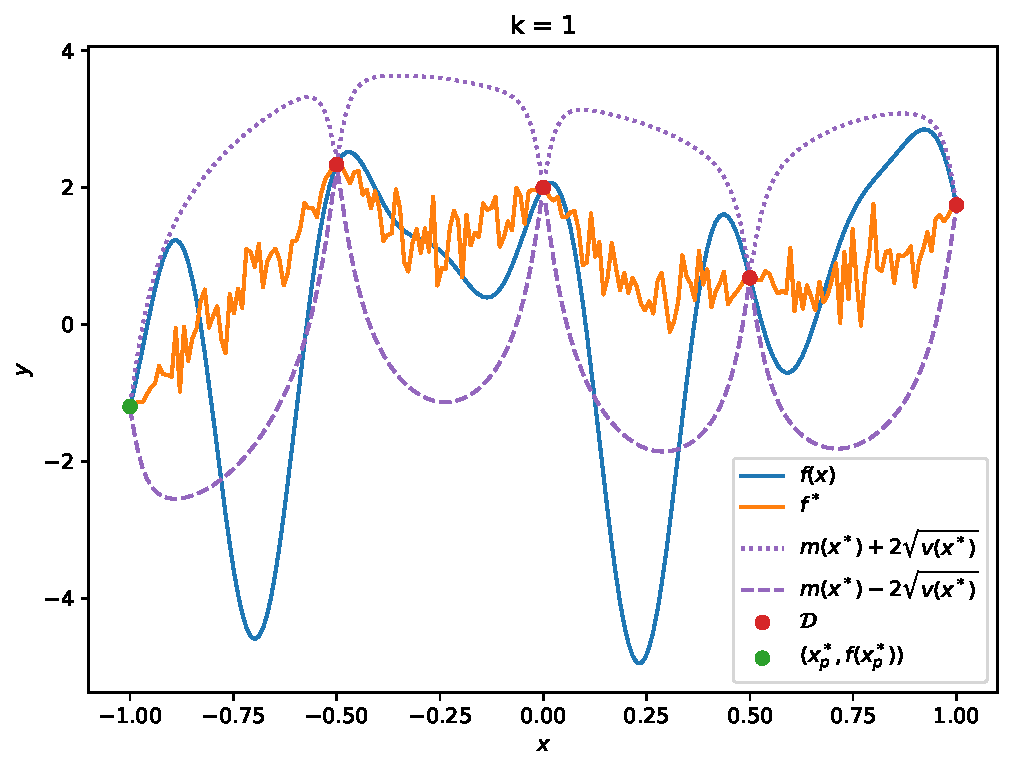
\includegraphics[width=\textwidth]{figures/gp/b2-k=1.pdf}
    \end{subfigure}
    \hfill
    \begin{subfigure}[t]{0.49\textwidth}
        \centering
        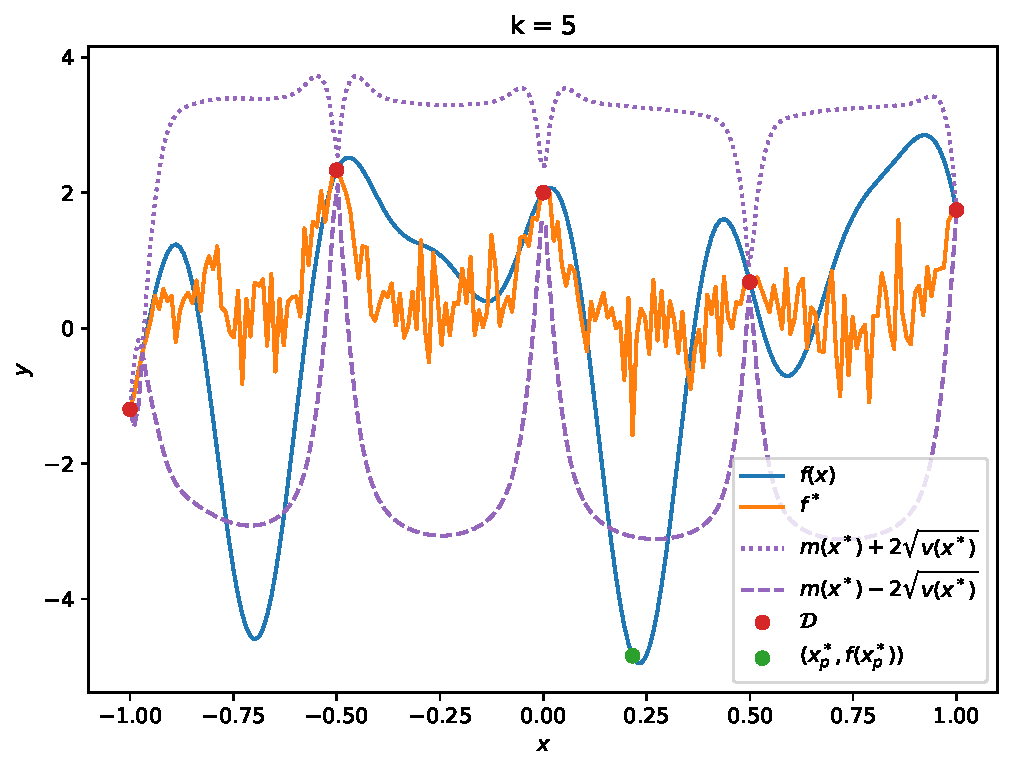
\includegraphics[width=\textwidth]{figures/gp/b2-k=5.pdf}
    \end{subfigure}

    \medskip
    
    \begin{subfigure}[t]{0.49\textwidth}
        \centering
        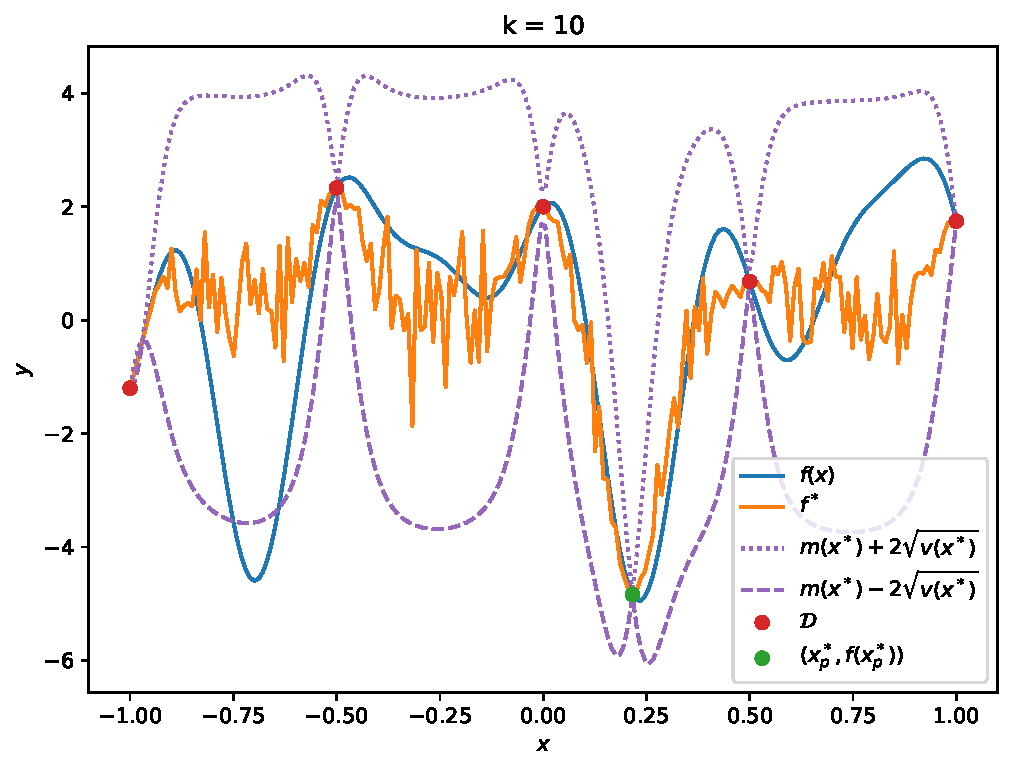
\includegraphics[width=\textwidth]{figures/gp/b2-k=10.pdf}
    \end{subfigure}
    \caption{Plots from running our Bayesian optimization loop at iteration $k$}
    \label{fig:gp:bayesianloop}
\end{figure}